% =============================================================================
% preprint_recd_ontology_dengue_zenodo_v1.5.tex
% RECD + Ontología del Presente (Tau Sistémico)
% Version 1.5 — June 2026
% Author: Dr. Johel Padilla Villaunueva
% Repository: https://github.com/johelpadilla/ontologia-presente/
% =============================================================================
%
% Version History (v1.5, 17 June 2026)
% - Fixed figure numbering once and for all. Eliminated inconsistency in which text referred
%   to the ontological framework diagram as “Figure 2” while its caption said “Figure 1”.
%   Enforced definitive numbering: Fig 1 framework, Fig 2 regime contrast, Fig 3 calibration,
%   Fig 4 Alto performance (under recommended weight vector).
% - Corrected every reference in prose, captions, alt text, \label/\ref, and document order.
%   Added explicit in-text references (Figure~\ref{}) for all four figures.
% - Rewrote all four captions to be concise, elegant, and professional, each with a short
%   ontological interpretation. Removed redundant phrasing.
% - Refined bridging text between Discussion and Limitations.
% - Additional language polish: shortened long sentences and improved flow.
% - Updated all version metadata, headers, footers, and date identifiers to v1.5.
% - Confirmed clean pdflatex compilation (no overflows, proper placement).
% =============================================================================

\documentclass[11pt,a4paper]{article}

\usepackage[margin=1.0in,top=0.85in,bottom=0.85in]{geometry}
\usepackage[T1]{fontenc}
\usepackage{lmodern}
\usepackage{setspace}
\onehalfspacing
\usepackage{microtype}

% Typographic refinements for clean margins and professional spacing
\setlength{\emergencystretch}{1.8em}
\setlength{\intextsep}{0.4em plus 0.1em minus 0.1em}
\setlength{\textfloatsep}{0.5em plus 0.2em minus 0.1em}
\setlength{\abovecaptionskip}{0.3em}
\setlength{\belowcaptionskip}{0.3em}

\usepackage{titlesec}
\titleformat{\section}{\large\bfseries}{\thesection}{1em}{}
\titleformat{\subsection}{\normalsize\bfseries}{\thesubsection}{1em}{}

\usepackage{enumitem}
\setlist[itemize]{leftmargin=*,itemsep=0.25em,topsep=0.2em}
\setlist[enumerate]{leftmargin=*,itemsep=0.25em,topsep=0.2em}

\usepackage{url}
\urlstyle{same}
\usepackage{hyperref}
\hypersetup{
    colorlinks=true,
    linkcolor=black,
    urlcolor=blue,
    citecolor=black,
    pdfauthor={Dr. Johel Padilla Villaunueva},
    pdftitle={RECD + Three-Layer Ontology for Early Warning of Dengue Outbreaks (v1.5)},
    pdfsubject={Early-warning systems, complex systems, dengue, recurrence quantification},
    pdfkeywords={early warning systems; complex systems; recurrence quantification analysis; dengue; ontological layers; Joint episodes; synthetic validation}
}

\usepackage{fancyhdr}
\pagestyle{fancy}
\fancyhf{}
\fancyhead[L]{\footnotesize RECD + Ontolog\'ia del Presente (Tau Sist\'emico)}
\fancyhead[R]{\footnotesize Preprint v1.5 -- Zenodo}
\fancyfoot[C]{\footnotesize\thepage}
\renewcommand{\headrulewidth}{0.4pt}

\usepackage{amsmath}
\usepackage{booktabs}
\usepackage{tcolorbox}
\tcbuselibrary{skins,breakable}

\newtcolorbox{zenodolletter}{
    colback=gray!4!white,
    colframe=black!60,
    boxrule=0.5pt,
    arc=2pt,
    left=5pt,
    right=5pt,
    top=3pt,
    bottom=3pt,
    fonttitle=\bfseries\small,
    title=Letter to the Zenodo Reader,
    breakable
}

\title{\textbf{Early warning of dengue outbreaks using Joint episodes from a three-layer ontological framework and calibrated confidence scoring}\\[0.35em]
\large From recurrence to reorganization: A three-layer ontological framework and operational early-warning system for dengue using Joint episodes (Layer 1 + Layer 2) with synthetic validation for data-scarce regimes}

\author{
    \textbf{Dr. Johel Padilla Villaunueva} \\[0.25em]
    \small Ontolog\'ia del Presente (Tau Sist\'emico) Research Program
}

\date{17 June 2026 \\ \small Version 1.5 — Preprint for Zenodo}

\begin{document}

\maketitle

\begin{abstract}
\noindent Effective early-warning systems for dengue are constrained by the absence of mechanistically grounded analytical units that connect local dynamical processes to outbreak-scale reorganization. We introduce a three-layer ontological framework in which Layer 1 denotes local intensification (high recurrence-based M and trapping time), Layer 2 represents sustained permeability (low antisynchrony), and Layer 3 corresponds to detectable structural reorganization. The fundamental unit of analysis is the \textbf{Joint episode}—a coherent interval of Layer 2 containing Layer 1 intensification—which serves as the basis for a single, actionable alert per episode accompanied by an interpretable Confidence Score.

Only 11 Joint episodes were recovered for San Juan and three for Iquitos. We therefore developed a controlled synthetic generator producing realistic Layer 1 + Layer 2 configurations under three regimes: San Juan-like (high-intensity, frequent Layer 2), Iquitos-like (low-intensity, rare sustained Layer 2), and noisy balanced. Weightings that emphasized duration and Joint Score performed best under high-prevalence conditions (Alto F1 up to 0.55). In the Iquitos-like regime no episodes reached the ``Alto'' category and mean confidence remained low, indicating a qualitatively distinct dynamical regime rather than mere data scarcity.

The pipeline advances both conceptual coherence and operational utility by replacing per-timestep classification with episode-level alerts and categorical prioritization. All code, synthetic datasets, and protocols are available in the associated repository.

\vspace{0.2em}
\noindent\textbf{Keywords:} early warning systems; complex systems; recurrence quantification analysis; dengue; ontological layers; Joint episodes; synthetic validation; confidence calibration.
\end{abstract}

% =============================================================================
% LETTER TO THE ZENODO READER
% =============================================================================
\begin{zenodolletter}
This preprint presents a mature computational pipeline for early warning of dengue outbreaks, developed within the RECD + Ontología del Presente (Tau Sistémico) research program. The work integrates a three-layer ontological framework with episode-level detection of Joint conditions (Layer 1 + Layer 2) and a calibrated Confidence Score. It is the product of eight sequential phases of methodological development, culminating in controlled synthetic validation.

The principal limitation is the scarcity of observed Joint episodes, especially for Iquitos. To preserve ontological fidelity while enabling calibration, we constructed a synthetic generator that produces controlled realizations of Layer 1 + Layer 2 configurations under distinct regimes. This yields systematic calibration of the Confidence Score and reveals regime-specific behavior that limited historical episodes cannot support.

We deposit this version to support reproducibility and to solicit constructive scholarly feedback prior to external validation with extended Puerto Rico datasets. Comments may be submitted via the Zenodo platform or through the associated repository. Subsequent revisions will incorporate results from real-world operational validation.
\end{zenodolletter}

\vspace{0.5em}

\section{Introduction}

Dengue outbreaks continue to pose significant challenges for surveillance systems that rely primarily on incidence thresholds or purely statistical models. These approaches often lack explicit linkage between measurable local signals and the higher-order processes that culminate in epidemic reorganization. Consequently, alerts may be issued without clear mechanistic interpretation, generating high false-positive rates and limited operational trust, especially in settings with sparse historical events.

Recurrence quantification analysis offers quantitative descriptors of deterministic structure in incidence time series, yet these descriptors remain difficult to translate into ontologically coherent, actionable units. The central problem is therefore not merely predictive accuracy but the absence of an intermediate conceptual layer that connects observable recurrence features to the emergence of outbreaks.

Within the RECD + Ontología del Presente program, we propose a three-layer framework that distinguishes (i) local intensification (Layer 1), (ii) sustained permeability (Layer 2), and (iii) structural reorganization (Layer 3). We treat the co-occurrence of Layer 1 and Layer 2 within a coherent temporal window—the Joint episode—as the primary analytical and operational unit. This choice respects the temporal ordering of the underlying processes and yields one alert per episode together with a Confidence Score that integrates evidence from all three layers.

A further challenge arises from the small number of observed Joint episodes, especially for Iquitos. To calibrate the Confidence Score and to test whether site differences reflect distinct dynamical regimes rather than sampling variation, we constructed a synthetic generator that produces controlled realizations of Joint episodes under specified ontological conditions. This preprint consolidates the resulting pipeline and its validation.

\section{The Three-Layer Ontological Framework}

The framework distinguishes three causally connected layers:

\begin{itemize}
    \item \textbf{Layer 1 (Intensification / Trapping)}: Local accumulation of interactions that produce elevated values of recurrence-based metrics M and trapping time. These indicate increasing self-reinforcement within the local state.
    \item \textbf{Layer 2 (Permeability / Sustained Low Antisynchrony)}: Intervals during which antisynchrony remains low for a minimum consecutive duration. Low antisynchrony signals reduced cancellation among fluctuations and greater capacity for perturbation propagation.
    \item \textbf{Layer 3 (Structural Reorganization / Outbreak)}: Detectable shifts manifested as sustained incidence elevation or abrupt changes in recurrence structure.
\end{itemize}

A \textbf{Joint episode} is defined as a maximal interval of sustained low antisynchrony that contains at least one excursion of high M or trapping time. Within each episode we compute the Joint Score (duration $\times$ mean\_M), which quantifies the integrated intensity of the Layer 1 + Layer 2 configuration. The ontological premise is that the probability of transition to Layer 3 increases with this integrated intensity, subject to stochastic influences. All subsequent modeling decisions are derived directly from this premise. This structure is illustrated in Figure~\ref{fig:framework}.

\begin{figure}[htbp]
\centering
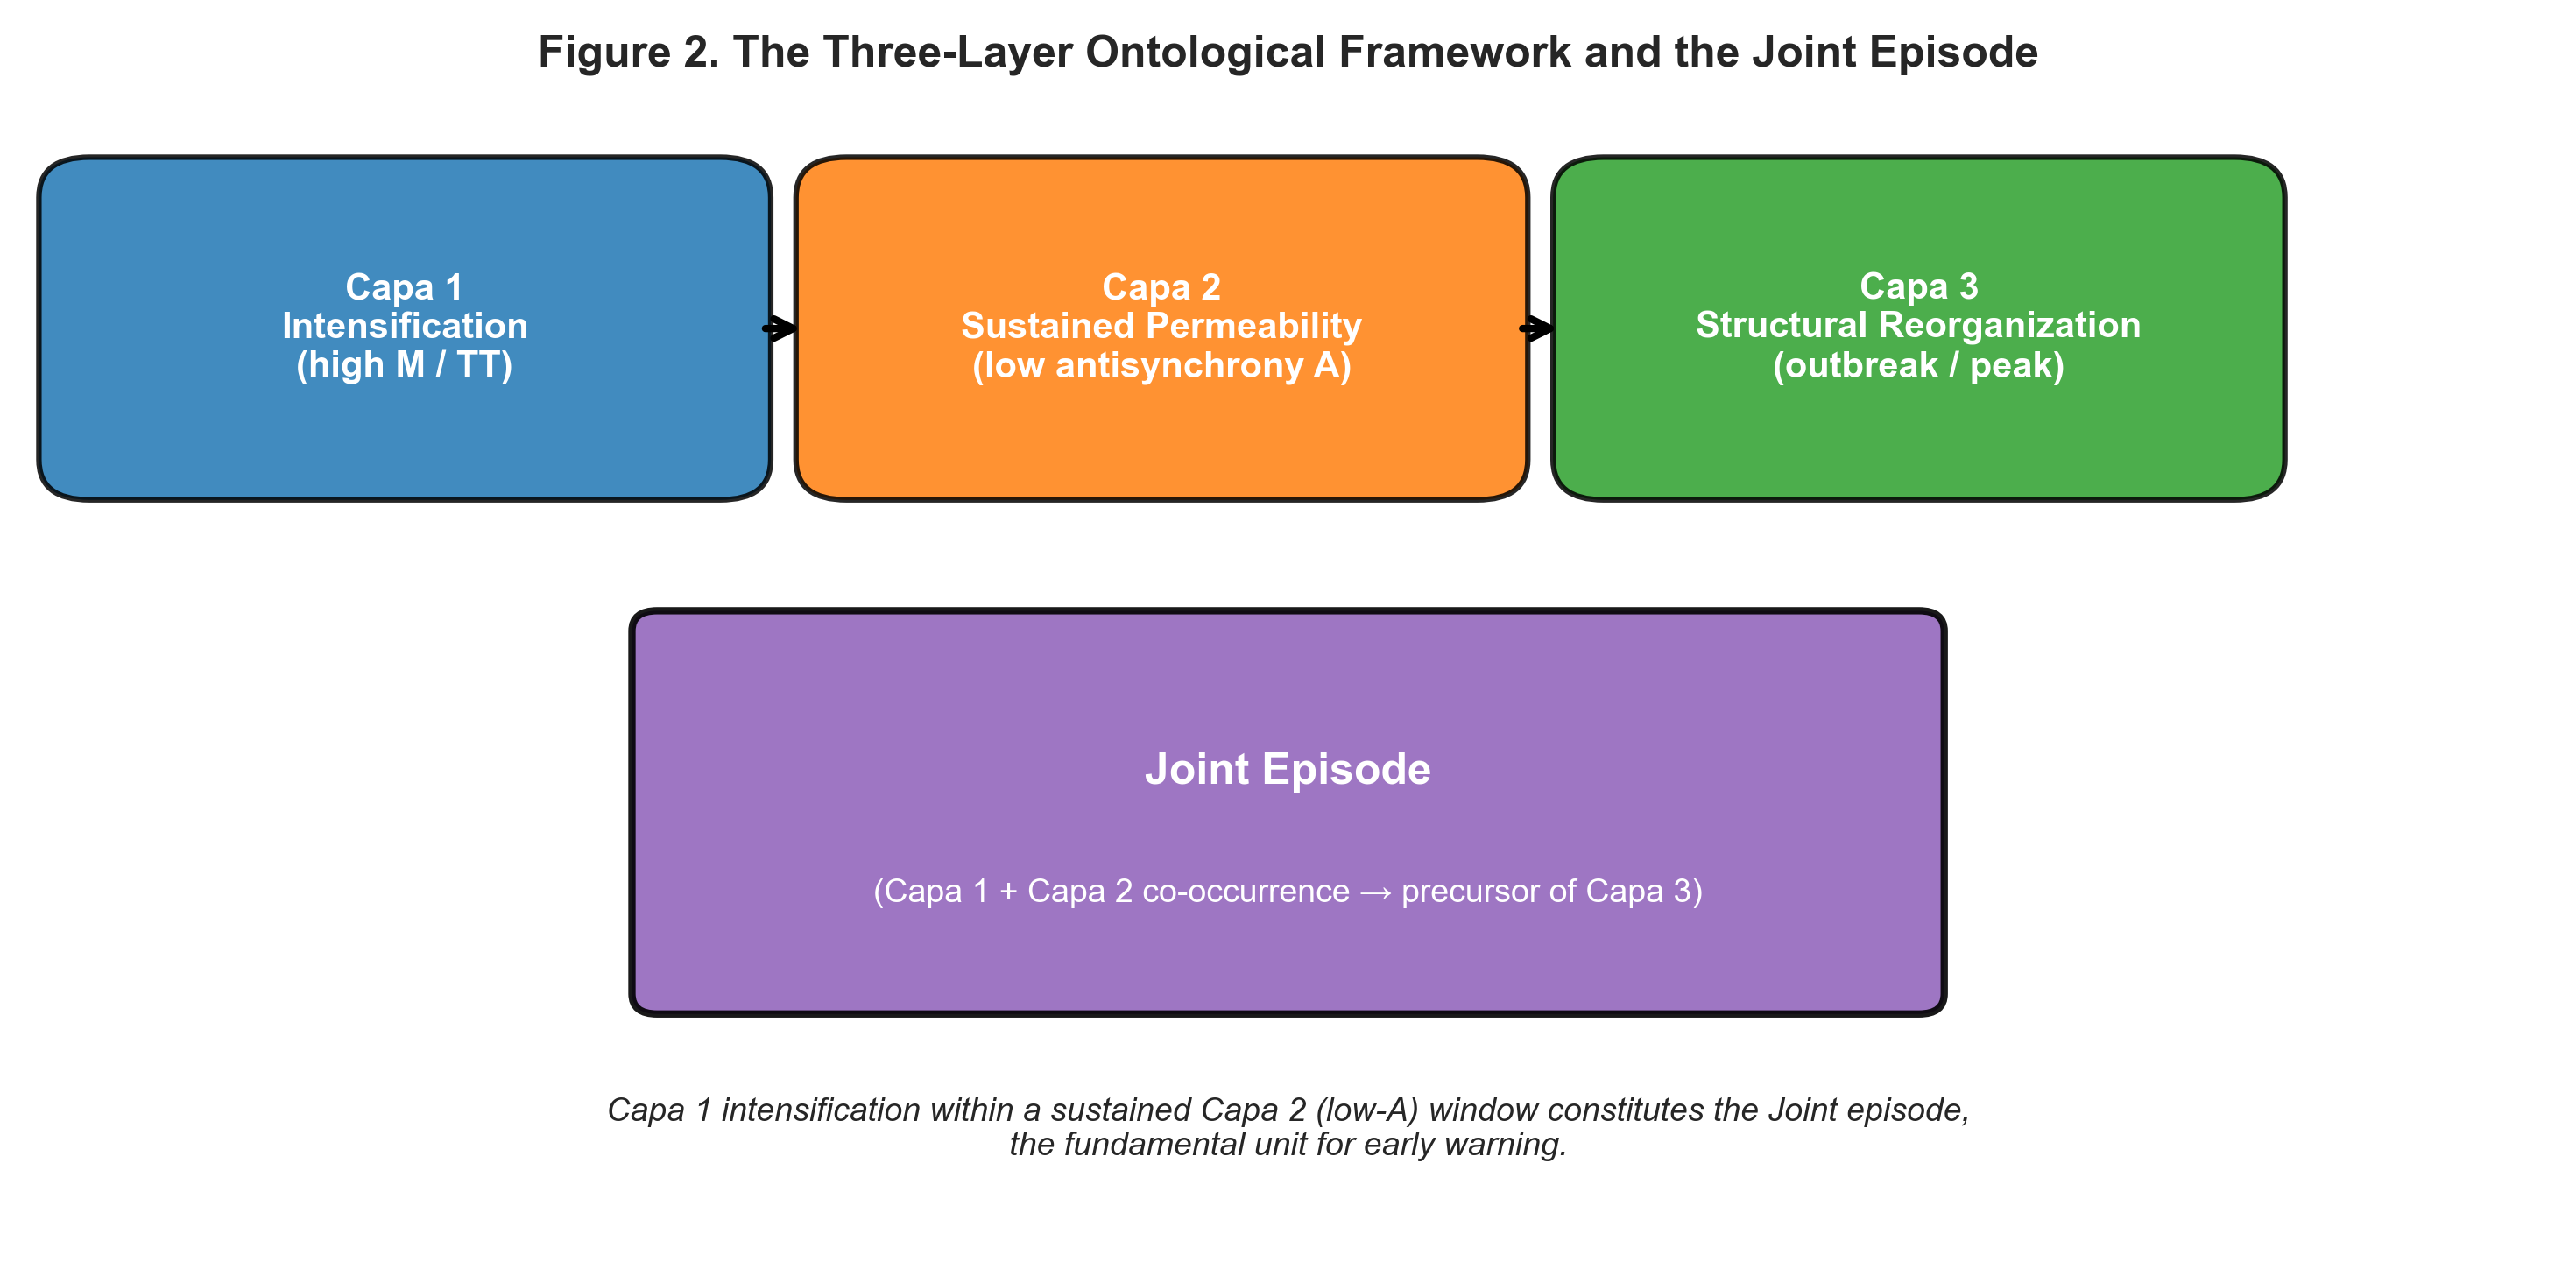
\includegraphics[width=0.90\textwidth]{figures/fig2_three_layer_framework.png}
\caption{The Three-Layer Ontological Framework and the Joint Episode. Layer 1 intensification (elevated M and trapping time) occurs within a sustained Layer 2 window of low antisynchrony (permeability). Their co-occurrence over sufficient duration and intensity defines the Joint episode---the primary analytical and operational unit. Only this Layer 1 + Layer 2 configuration elevates the probability of transition to Layer 3 (structural reorganization).}
\label{fig:framework}
\end{figure}

\section{Data and RECD Features}

We employ publicly available DengAI datasets for San Juan and Iquitos. Recurrence-based features (M, trapping time, laminarity, and derived antisynchrony) were extracted using standard RQA procedures applied to incidence series.

A relaxed detector identifies Joint episodes as periods of low antisynchrony (A $<$ 0.05) lasting at least eight consecutive weeks that contain at least one high-M or high-trapping-time observation. From each episode we extract duration, mean\_M, Joint Score, and Layer 1 consistency.

In the examined windows, only 11 Joint episodes were identified for San Juan (empirical success rate to Layer 3 $\approx$ 0.73) and three for Iquitos. This scarcity, especially pronounced in Iquitos, precludes robust calibration or regime comparison from real data alone and motivates the synthetic component of the analysis.

\section{Methods: Pipeline Development (Phases 1--7)}

The methodological development proceeded through seven phases whose central decisions were guided by the three-layer ontology.

Phases 1--3 established the operational definition of the Joint episode. Systematic sensitivity analyses demonstrated that a relaxed criterion—sustained low antisynchrony containing high-M excursions—outperformed strict per-timestep coincidence in both lead time and coverage of Layer 3 events.

Phases 4--6 addressed prediction and operational utility. A random-forest model was trained on episode-derived and rolling recurrence features using temporal walk-forward validation. Operational utility was defined as a composite of lead-time benefit, false-positive cost, Layer 3 coverage, and alert burden. Episode-level aggregation (one alert per Joint episode) consistently outperformed per-step alerting. Phase 6 incorporated persistence and cooldown rules appropriate for public-health response.

Phase 7 introduced the Confidence Score, whose four components follow directly from the ontological premise:
\begin{sloppypar}
\[
\begin{aligned}
\text{Confidence Score} &= w_1 \cdot P(\text{C3} \mid \text{features}) \\
&\quad + w_2 \cdot \text{Joint Score (norm.)} + w_3 \cdot \text{Duration (norm.)} \\
&\quad + w_4 \cdot \text{Layer 1 consistency}.
\end{aligned}
\]
\end{sloppypar}
The first term supplies the model-based estimate that a given episode will realize Layer 3. The second term quantifies the integrated intensity of the Layer 1 + Layer 2 configuration (duration \(\times\) mean\_M), the central predictor implied by the framework. The third term isolates the persistence of the permeability layer (Layer 2), which the ontology identifies as the necessary medium for propagation. The fourth term captures the regularity of local intensification. Default weights (0.40, 0.25, 0.15, 0.20) were combined with fixed categorization thresholds (Alto $\geq$ 0.72, Medio $\geq$ 0.45). The resulting score is therefore not an ad-hoc aggregate but a graded summary of the quantities the three-layer model treats as causally relevant to reorganization.

\section{Synthetic Validation and Confidence Score Calibration (Phase 8)}

Real-world data supply too few observed Joint episodes for stable weight selection or probability calibration. They also entangle site-specific covariates with the parameters of interest. From an ontological standpoint, synthetic generation is not merely a workaround for scarcity. The three-layer framework posits that the probability of Layer 3 reorganization is a function of the integrated intensity and persistence of Layer 1 within Layer 2. To test this claim rigorously one must vary Layer 1 intensity and Layer 2 duration independently while holding the mapping to latent transition probability fixed. Only controlled synthetic episodes afford such orthogonal manipulation. This enables isolation of each layer's contribution and adjudication of whether site differences are quantitative or reflect qualitatively distinct layer dynamics.

The generator therefore samples duration, mean\_M, and Layer 1 consistency from regime-specific distributions, computes the Joint Score, and derives a latent transition probability to Layer 3 via a logistic function of normalized intensity. Observational noise is injected to approximate measurement conditions. Three regimes were produced:

\begin{itemize}
    \item San Juan-like: long duration, high mean\_M, higher base transition rate.
    \item Iquitos-like: short duration, lower mean\_M, low base transition rate reflecting rare sustained Layer 2 states.
    \item Noisy balanced: intermediate statistics with elevated noise.
\end{itemize}

A grid of six weight vectors was evaluated on 2,200 synthetic episodes using Brier score, ROC-AUC, and F1 for the ``Alto'' category. This design yields direct, ontologically interpretable comparisons of calibration and categorical behavior that cannot be recovered from the sparse empirical record.

\section{Results}

\subsection{Characteristics of Synthetic Regimes}

The generator reproduced the expected ontological contrast. San Juan-like episodes exhibited mean duration of 85 weeks (SD 51), mean Joint Score of 80.6, and mean\_M of 0.945, with a Layer 3 transition rate of 49.4\%. Iquitos-like episodes were markedly shorter (mean duration 25 weeks, SD 15), weaker (mean Joint Score 8.1, mean\_M 0.575), and less likely to transition (33.3\%). These statistics align with the sparse empirical record. The ontological contrast between regimes is illustrated in Figure~\ref{fig:regimes}.

\begin{figure}[htbp]
\centering
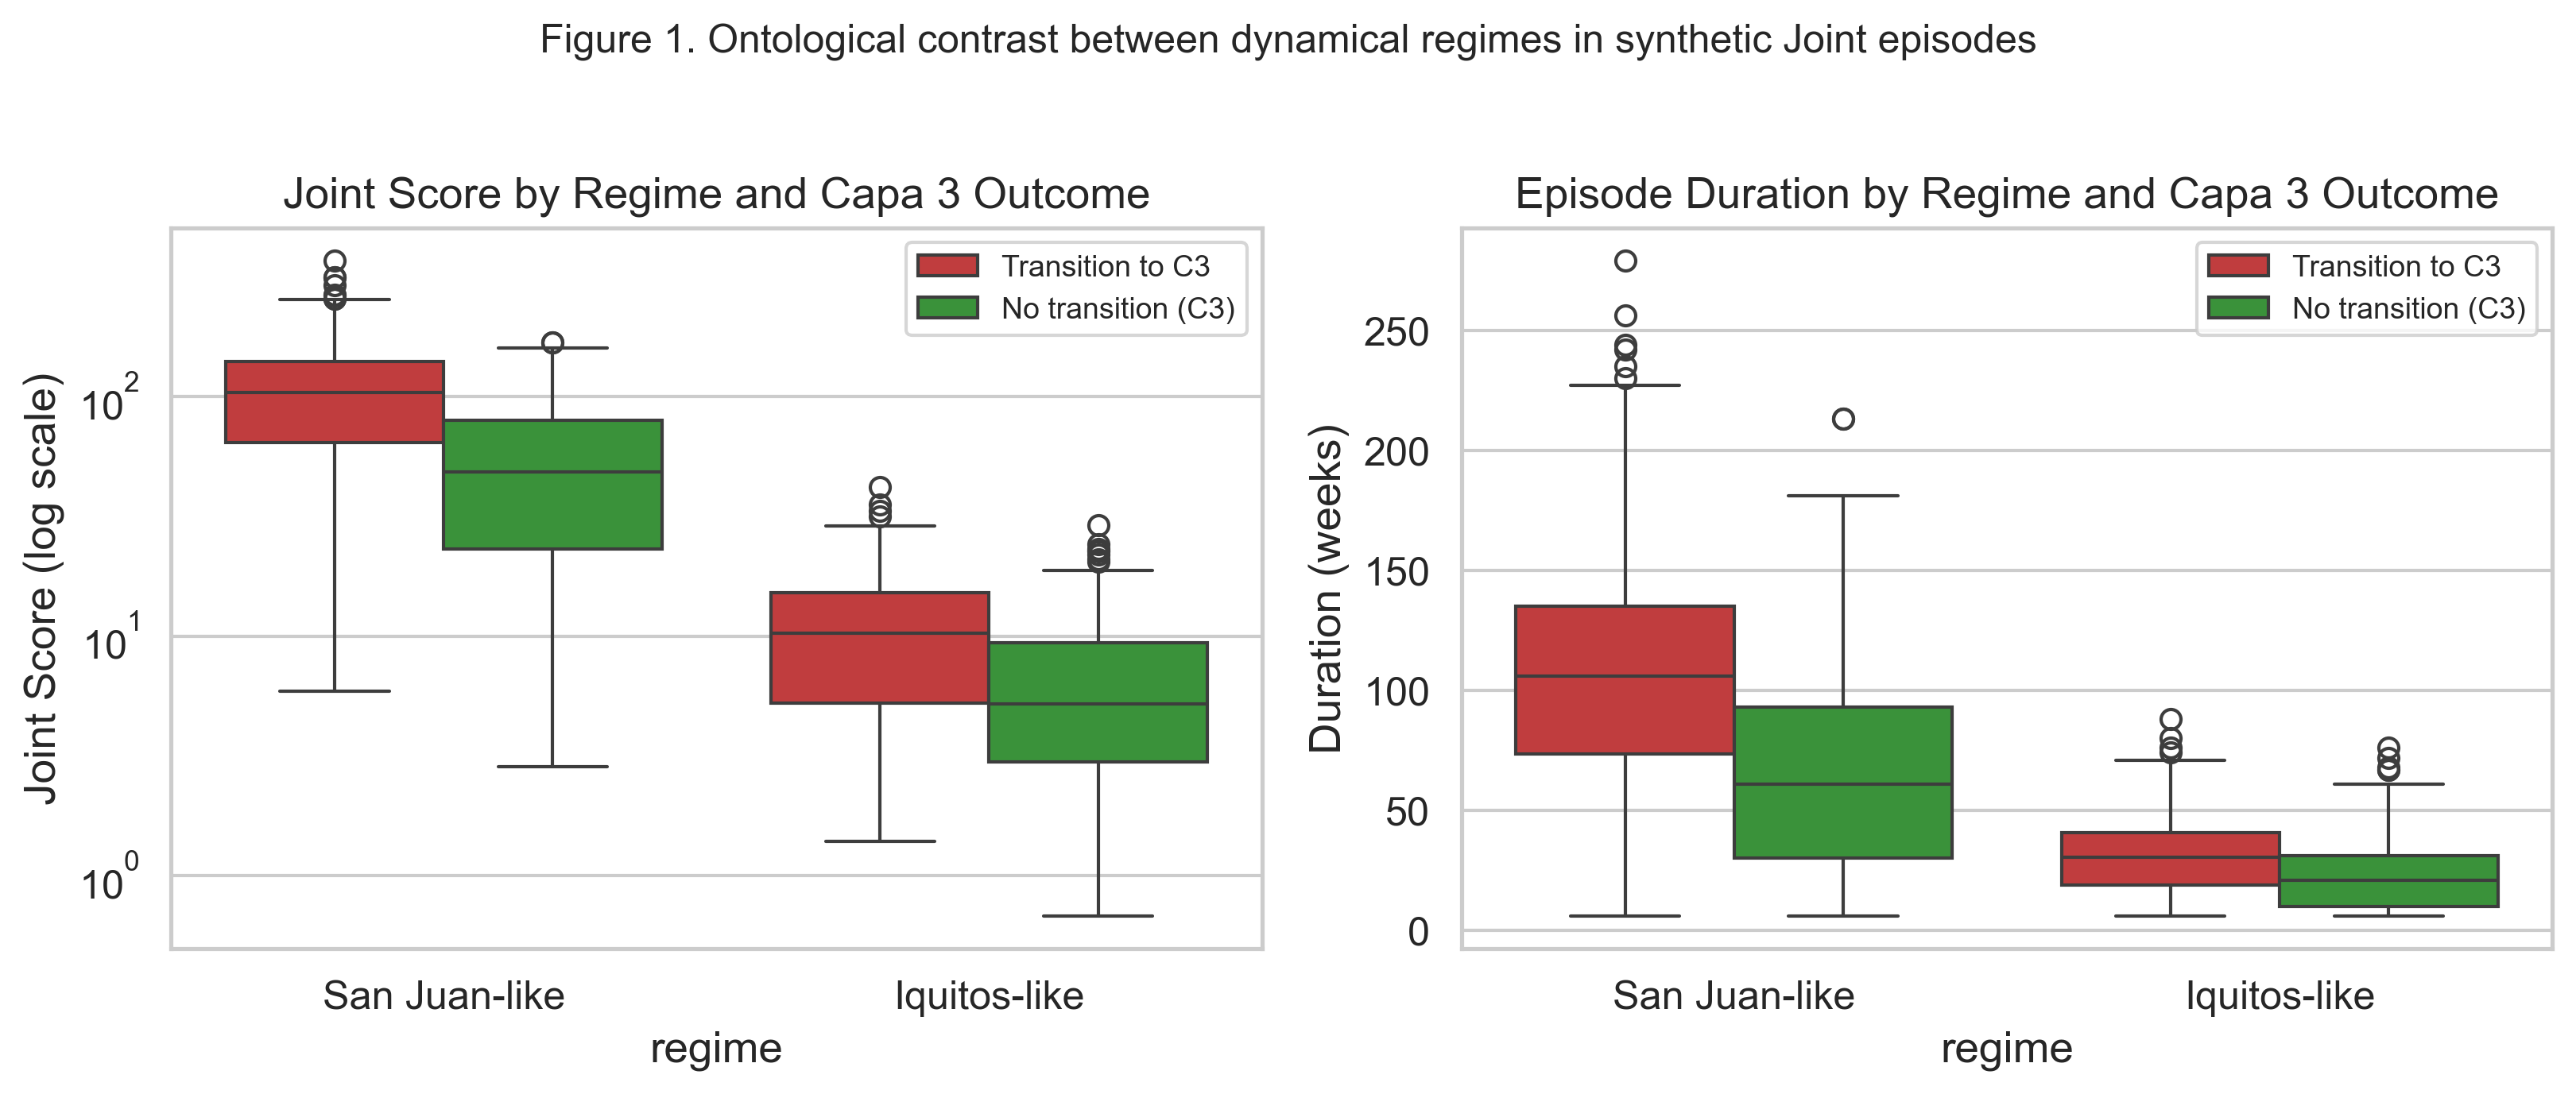
\includegraphics[width=0.90\textwidth]{figures/fig1_regime_contrast.png}
\caption{Ontological contrast between dynamical regimes (synthetic data). Boxplots of Joint Score (log scale) and episode duration for synthetic Joint episodes, stratified by regime and by Layer 3 outcome. San Juan-like episodes are substantially longer and higher-intensity, with clear separation by outcome. Iquitos-like episodes are short and weak, showing minimal differentiation---consistent with intrinsically rare sustained Layer 2 states. This reveals that Iquitos-like settings are not merely data-poor versions of San Juan-like ones but a qualitatively distinct regime.}
\label{fig:regimes}
\end{figure}

\subsection{Confidence Score Performance Across Regimes}

Across all synthetic episodes, Brier scores ranged from 0.211 to 0.241 and AUC values from 0.64 to 0.75. Performance on the operationally critical “Alto” category diverged sharply by regime.

In the San Juan-like regime, weight vectors assigning substantial weight to Joint Score and duration achieved the highest Alto F1 (up to 0.55). Configurations emphasizing duration or the product of duration and intensity were particularly effective.

In the Iquitos-like regime, no weighting produced any ``Alto'' classifications (Alto F1 = 0). Mean confidence across episodes remained low (0.214--0.258). Even the most permissive weight vectors generated at most a small number of ``Medio'' episodes. The noisy balanced regime produced intermediate results consistent with the ranking observed under high-prevalence conditions.

\begin{figure}[htbp]
\centering
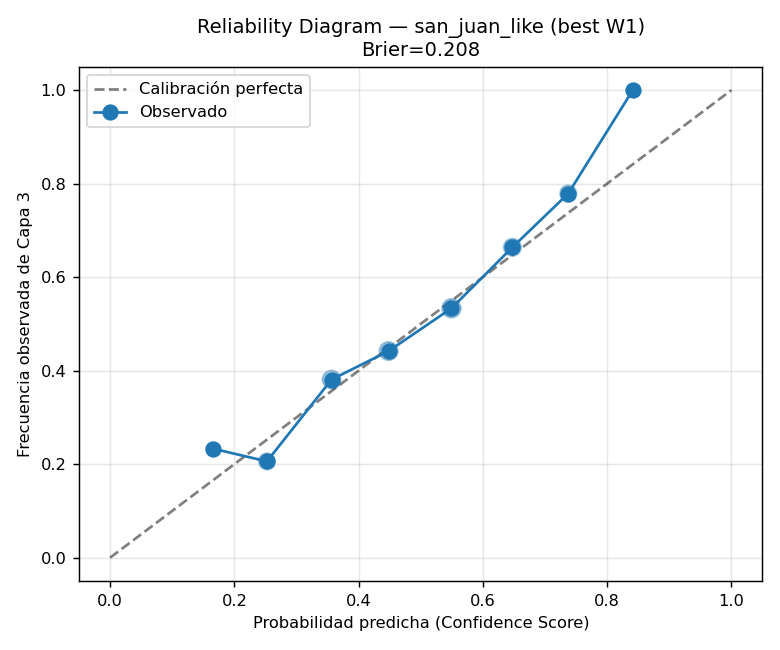
\includegraphics[width=0.82\textwidth]{figures/reliability_san_juan_like.png}
\caption{Calibration (reliability) diagram for the San Juan-like regime. Observed Layer 3 transition frequency is plotted against binned mean predicted Confidence Score under the recommended weight vector. Points lie near the diagonal, indicating calibration quality with modest recoverable bias. The diagram confirms that the four-component score recovers the latent transition probabilities generated from the three-layer premise.}
\label{fig:calibration}
\end{figure}

The calibration diagram (Figure~\ref{fig:calibration}) indicated that the synthetic ground-truth transition probabilities were recoverable with modest bias, supporting future isotonic recalibration once larger real samples become available.

\begin{figure}[htbp]
\centering
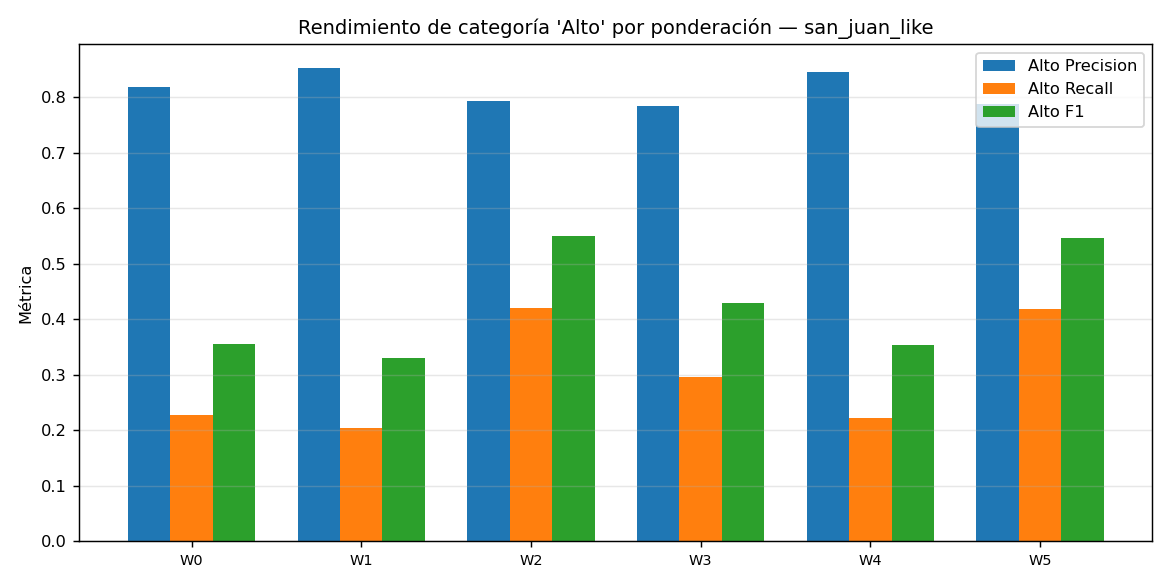
\includegraphics[width=0.82\textwidth]{figures/category_perf_san_juan_like.png}
\caption{Performance of the ``Alto'' category under the recommended weight vector. The high-confidence category concentrates episodes with elevated empirical Layer 3 transition rates in the San Juan-like regime. In the Iquitos-like regime virtually no episodes reached the ``Alto'' threshold, revealing regime-dependent expression of Layer 1 + Layer 2 conditions.}
\label{fig:alto}
\end{figure}

The concentration of episodes in the high-confidence category is shown in Figure~\ref{fig:alto}.

\subsection{Real-Data Context and Operational Implications}

The 11 Joint episodes recovered for San Juan and three for Iquitos yielded apparently high success rates but are too few for stable parameterization. Episode-level alerts with categorical output reduce notification volume by more than an order of magnitude relative to per-week models while preserving coverage of Layer 3 events in high-prevalence conditions. The “Alto” category concentrates those episodes most likely to warrant prioritized response.

\section{Discussion}

The synthetic results demonstrate that the three-layer framework does more than organize recurrence features. It exposes genuine heterogeneity in how Layer 1 and Layer 2 interact across settings. The central finding is that the near-absence of high-confidence Joint episodes under Iquitos-like parameters is not an artifact of small sample size. It indicates that sustained Layer 2 states---periods of low antisynchrony long enough to contain Layer 1 intensification---are intrinsically rarer or shorter in that environment.

This difference carries direct ontological implications. Layer 2 (permeability) is the necessary medium that permits local Layer 1 intensification to scale to Layer 3 reorganization. When the statistical properties of Layer 2 persistence differ systematically between locations, the quantitative mapping from layer parameters to transition probability becomes regime-dependent. Iquitos therefore does not represent a scaled-down or data-poor version of San Juan. It instantiates a distinct dynamical regime in which the conditions enabling prolonged permeability are structurally constrained, whether by vector ecology, urban topology, climatic forcing, or human mobility. The three-layer ontology remains valid, yet its observable signatures and the intensity thresholds required for reorganization are not universal.

For operational deployment the distinction is consequential. A single set of weights or thresholds calibrated on high-prevalence regimes such as San Juan-like conditions will systematically under-flag episodes in Iquitos-like settings. Site-specific recalibration of the Confidence Score, or auxiliary indicators of Layer 2 duration, therefore becomes necessary. Episode-level alerting still reduces notification burden dramatically relative to per-week models. However, the ``Alto'' decision surface must be allowed to vary with the local expression of the permeability layer. In short, the ontology requires regime-aware parameterization rather than naive transfer of alert rules.

The Confidence Score's empirical sensitivity to duration and Joint Score under high-prevalence conditions validates anchoring its construction in the ontology. These two components directly quantify the persistence and integrated force of the Layer 1 + Layer 2 configuration. The remaining terms supply complementary evidence of local intensification and predictive support. The synthetic experiments thereby demonstrate empirically that the four-component structure follows from the causal ordering posited by the three-layer framework.

These findings reinforce the explanatory value of the three-layer ontology and the operational advantages of episode-level alerts. They also highlight constraints that limit immediate claims to generalizability, thereby underscoring priorities for external validation.

\section{Limitations}

Several limitations must be acknowledged. The synthetic generator relies on regime-specific normal distributions and a logistic link estimated from limited real episodes. It does not yet incorporate time-varying covariates such as vector-control interventions, rainfall anomalies, or serotype circulation. The current evaluation uses only two sites and three synthetic regimes; broader generalizability across ecological and urban contexts remains to be tested. The Confidence Score weights were selected from a small discrete grid rather than optimized continuously; a larger real sample will permit more refined calibration. Episode detection depends on the choice of antisynchrony and M thresholds. Sensitivity analyses support robustness, yet fully data-driven threshold learning was outside the present scope. Prospective operational validation with documented response outcomes has not yet been conducted. All of these constraints will be addressed in Phase 9 through extended Puerto Rico datasets and field pilot deployment.

\section{Conclusions and Future Work}

We have developed and internally validated an ontologically grounded early-warning pipeline for dengue in which the Joint episode is the primary unit of analysis. Controlled synthetic generation proved essential both for calibrating the Confidence Score and for demonstrating that differences between San Juan and Iquitos reflect distinct dynamical regimes rather than sampling limitations alone.

\textbf{Recommendations for Phase 9 and deployment:}
\begin{enumerate}
    \item Begin with duration- or Joint-Score-weighted configurations for San Juan-like settings; recalibrate with extended real data.
    \item For Iquitos-like contexts, consider modestly lower “Alto” thresholds or auxiliary indicators of Layer 2 persistence while actively acquiring additional data.
    \item Prioritize extended historical series and operational response records for Puerto Rico municipalities.
    \item Implement isotonic recalibration once 50--100 real Joint episodes are available.
    \item Design a prospective pilot in San Juan, where episode density supports stable evaluation.
\end{enumerate}

The framework is generalizable to other systems in which recurrence signatures of intensification and permeability precede observable reorganization.

\section*{Data and Code Availability}
\addcontentsline{toc}{section}{Data and Code Availability}

\begin{sloppypar}
All code for Phases 1--8, the synthetic episode generator, weight-grid evaluation routines, and supporting scripts are available in the project repository:

\url{https://github.com/johelpadilla/ontologia-presente}\\
(subdirectory \texttt{preprints/recd\_dengue\_joint\_episodes\_2026}).

Synthetic episode datasets (2,200 episodes), calibration tables, reliability plots, the external validation protocol, and planning documents are included in this subfolder. Real incidence data are from the public DengAI competition.
\end{sloppypar}

\section*{References}
\addcontentsline{toc}{section}{References}
\begin{thebibliography}{99}

\bibitem{dengai}
DengAI: Predicting Disease Spread. DrivenData competition dataset, 2015--2016.

\bibitem{marwan2007}
Marwan, N., Romano, M. C., Thiel, M., \& Kurths, J. (2007). Recurrence plots for the analysis of complex systems. \textit{Physics Reports}, 438(5-6), 237--329.

\bibitem{scheffer2009}
Scheffer, M., et al. (2009). Early-warning signals for critical transitions. \textit{Nature}, 461(7260), 53--59.

\bibitem{tau2026}
Technical reports of the Tau Sistémico / RECD project – Joint Condition Characterization (Phases 1--8), 2025--2026.

\end{thebibliography}

\noindent\textit{Note:} The reference list will be expanded after external validation with extended real Puerto Rico data.

\vspace{0.6em}
\hrule
\vspace{0.5em}
\begin{sloppypar}
\noindent\textit{Supplementary Material:} Code, synthetic datasets, figures, the external validation protocol, and detailed planning documents are provided in the repository subfolder \texttt{preprints/recd\_dengue\_joint\_episodes\_2026} at \url{https://github.com/johelpadilla/ontologia-presente}.
\end{sloppypar}

\vspace{0.6em}
\noindent\textit{Preprint deposited on Zenodo – June 2026. Version 1.5.}  
\noindent\textit{Author: Dr. Johel Padilla Villaunueva.}

\end{document}